\section{Procesní model a důvody pro jeho tvorbu}
Ať už člověk vytváří jakýkoliv model, jeho cílem je zachytit nějaký jev, který je potřeba kvůli své komplexnosti zobrazit zjednodušenou vizuální formou, která bude pochopitelná i pro jiné lidi než je sám tvůrce modelu. Umět jev zachytit ve formě modelu je jedním z prvních kroků na cestě k tomu tento jev upravovat.

Přeneseno do světa podnikových procesů je situace velmi podobná. Jedním z hlavních důvodů, proč organizace přistupují k BPM je potřeba procesy upravovat a zejména optimalizovat. Aby to bylo možné, je potřeba nejdřív stanovit metriky a tyto metriky být pak schopen měřit. Základem pro všechny tyto kroky je ale korektní procesní model, který proces věrně popisuje.

\subsection{Definice procesního modelu}
Základní definice procesního modelu podle \cite{Dietz2006}:
\begin{quote}
Procesní model je konceptualizací podnikového procesu v organizaci.
\footnote{Process model is a conceptualization of the (business) process in an enterprise. \cite{Dietz2006}}
\end{quote}
Čtenářsky přístupnější definici pak nabízí \cite{Recker2009}:
\begin{quote}
Procesní model popisuje (většinou grafickou formou) aktivity, události, jejich pořadí a propojení, které utváří podnikový proces.
\footnote{Process model describe, typically in a graphical way, the activities, events and control flow logic that constitues a business process.}
\end{quote}

\section{Základní techniky}
V této sekci si popíšeme populární techniky pro tvorbu procesních modelů.

\subsection{Vývojový diagram (Flowchart)}
\textit{Vývojový diagram} je pravděpodobně nejpopulárnější technikou pro modelování podnikových procesů. Vděčí za to zejména své jednoduchosti, dostupnosti mnoha nástrojů, které tuto techniku podporují a také její velké srozumitelnosti, která jí činí velmi snadno uchopitelnou i pro ty uživatele v organizaci, kteří nejsou příliš obeznámeni s problematikou modelování podnikových procesů.

\subsubsection{Základní pravidla}
Vývojové diagramy se skládají z několika málo základních symbolů. Tyto symboly se nazývají: \cite{Chytil2005}

\begin{itemize}
\item \textit{Startovací a ukončovací symboly} – používají se pro vyznačení začátku a konce procesu.
\item \textit{Šipky} – zobrazují tzv. \uv{řídící tok}, tedy přechod v čase mezi jednotlivými symboly.
\item \textit{Dílčí kroky procesu} – jsou reprezentovány obdélníkem.
\item \textit{Podprogramy} – zobrazeny obdélníkem se svislými čarami po stranách. Používají se pro zobrazení skupiny kroků procesu pomocí jediného symbolu.
\item \textit{Vstupy a výstupy} – zobrazují tok informací směrem dovnitř i vně procesu. Pro jejich reprezentaci se používají lichoběžníky respektive rovnoběžníky.
\item \textit{Podmíněný cyklus} – zobrazuje událost, která se opakuje dokud je splněna jasně definovaná podmínka. Zobrazuje se pomocí šestiúhelníku.
\item \textit{Podmíněný výraz} – kosočtvercem je symbolizováno rozhodnutí a určuje tedy místo, kde dochází k větvení procesu.
\item \textit{Spojovací symbol} – inverzním symbolem ke kosočtverci je ve vývojovém diagramu kruh, který se používá ke spojení více řídících toků do jednoho.
\end{itemize}

\begin{figure}[H]\centering %todo překreslit obrázek%
\includegraphics[width=1.0\textwidth]{obrazky/flowchart}
\caption{Nákupní proces pomocí vývojového diagramu}
\label{fig:Flowchart}
\end{figure}

\subsubsection{Výhody a nevýhody}
Nespornou výhodou vývojových diagramů je právě jejich přístupnost pro uživatele a velmi strmá křivka učení, což dělá z této techniky první volbu pro případy, kdy je potřeba velmi rychle vymodelovat nějaký proces a organizace nemá zavedeny sofistikovanější metody BPM. Vývojové diagramy umožňují efektivnější komunikaci o problému v rámci týmu. 

Největší přednost vývojových diagramů je zároveň jejich největší slabinou. Právě přílišná jednoduchost této techniky dělá z modelování komplexnějších procesů poměrně komplikovanou a nepřehlednou záležitost. Ve vývojových diagramech je také složitější modelovat některé jevy, jako například tzv. \uv{unhappy paths} a další nestandardní události, která však v životě procesů nastávají poměrně běžně. U vývojových diagramů je také obtížné dělat změny, protože to často vyžaduje kompletní překreslení celého diagramu.

\subsubsection{Použití}
Vývojové diagramy mají mnoho využití. Hodí se například pro komunikaci mezi organizací a jejími externími zákazníky, protože se dá předpokládat, že se s vývojovými diagramy už v minulosti setkali a budou jim tedy rozumět. Vhodné je také použít vývojový diagram v dokumentaci k softwaru nebo jinému systému, kterou budou číst různorodé skupiny uživatelů.

\subsection{BPMN}
\textit{BPMN} nebo celým názvem \textit{Business Process Model and Notation} je v současnosti de facto standardem na poli modelování podnikových procesů. Jeho využití je široké od IT přes obchod až například po komplexní dopravní systémy. Za svou popularitu vděčí zejména tomu, že se stále jedná o dobře pochopitelnou grafickou notaci, která je svým vzhledem velmi podobná vývojovým diagramům, ale na rozdíl od nich je BPMN standardem, tedy má oficiální specifikaci s popisem jednotlivých elementů a pravidel, jak je používat.

S trochou nadsázky by se dalo říct, že BPMN je vlastně rozšířením vývojového diagramu. Je určitě pravdou, že se BPMN touto jednoduchou technikou v mnohém inspirovalo a na jejích základech postavilo notaci, která umožňuje poměrně jednoduše modelovat i komplexní podnikové procesy a zároveň si stále uchovává dobrou srozumitelnost pro uživatele.

\subsubsection{Základní pravidla}
Jelikož se BPMN budeme podrobně věnovat v kapitole 3 %todo odkaz%
nemá smysl na tomto místě zacházet do přílišných detailů. Zatím si vystačíme s tím, že v BPMN jsou zásadními objekty \textit{aktivity}, \textit{události}, \textit{brány}, \textit{počáteční a koncové symboly} a \textit{\uv{šipky}} neboli symboly reprezentující \textit{sekvenční tok} procesu nebo zasílání \textit{zpráv}. Vzhledově se tyto symboly příliš neliší od korespondujících  symbolů ve vývojovém diagramu.

\begin{figure}[H]\centering 
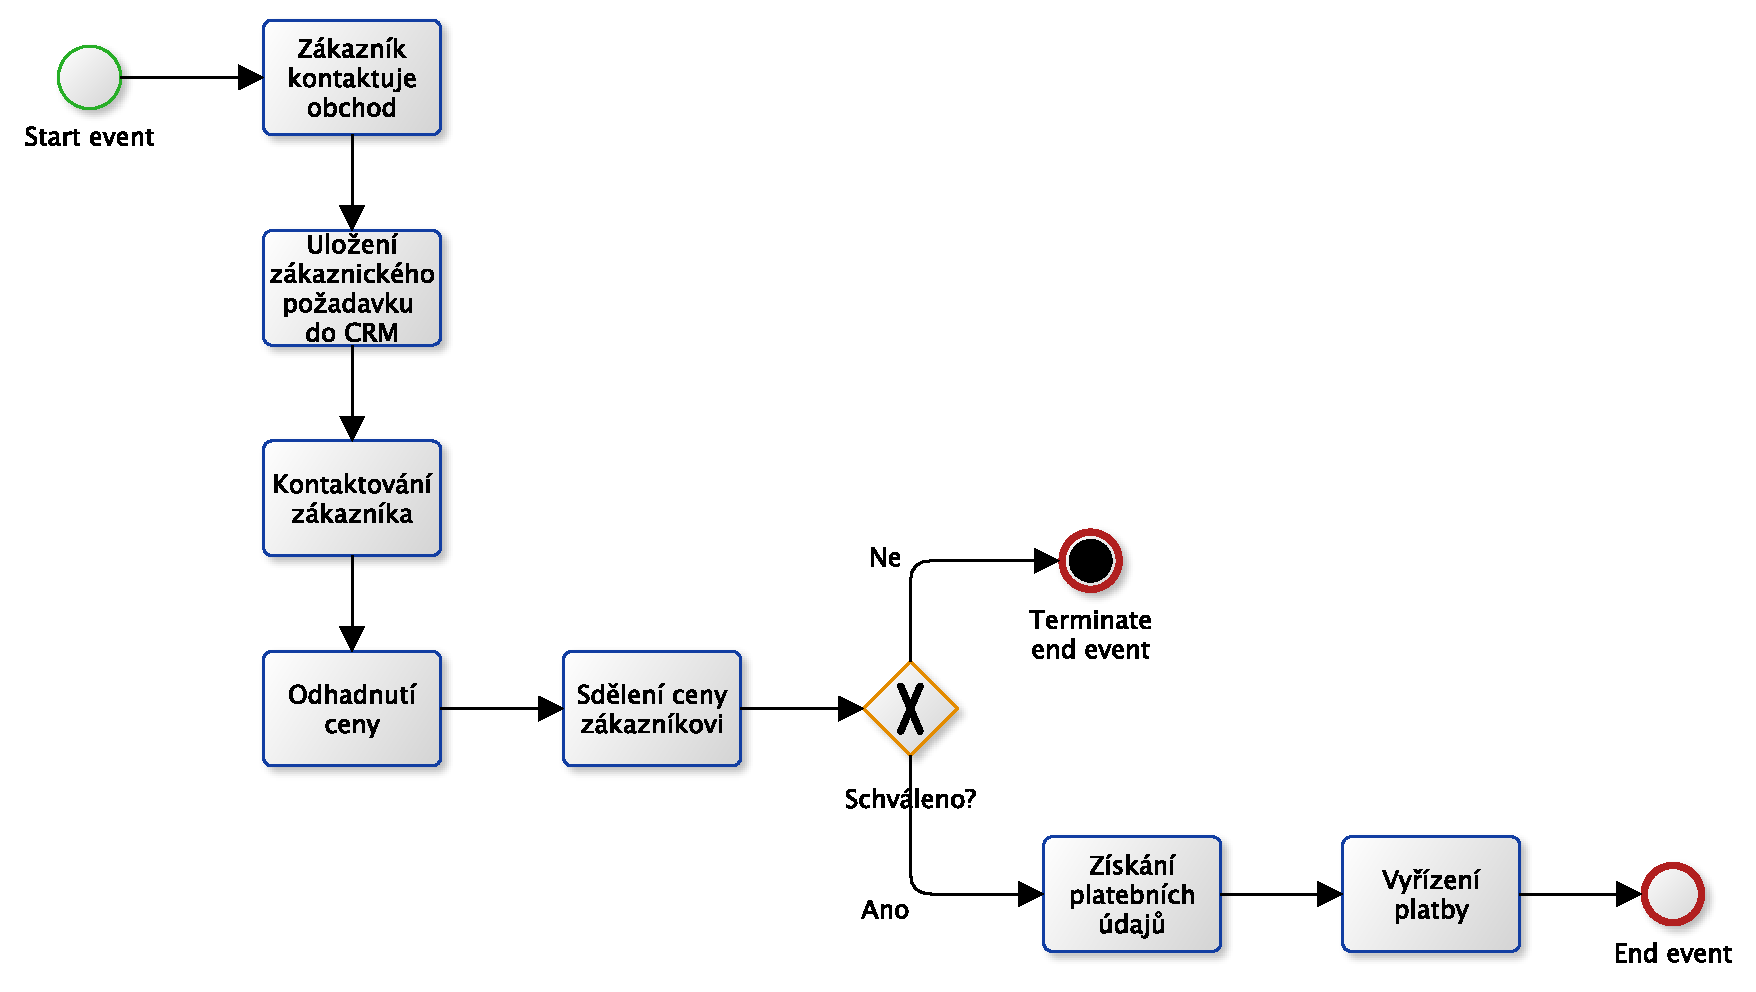
\includegraphics[width=1.0\textwidth]{obrazky/bpmn-order-process}
\caption{Nákupní proces pomocí BPMN}
\label{fig:BPMN_nakupniproces}
\end{figure}

\subsubsection{Výhody a nevýhody}
Mezi hlavní výhody BPMN určitě můžeme zařadit fakt, že BPMN je \textit{standard}, tedy je přesně definované, co který symbol vyjadřuje. O BPMN se stará organizace OMG (Object Management Group) a kontinuálně pracuje na jeho rozvoji. Díky širokému rozšíření BPMN existuje na trhu velké množství placených i neplacených nástrojů, které umožňují modelování podnikových procesů pomocí této notace.

Další neoddiskutovatelnou předností je srozumitelnost notace, která je vysoká právě díky své podobnosti s vývojovými diagramy. Bez nutnosti zdlouhavého studia dokumentace je BPMN modelu schopen porozumět člověk z managementu společnosti a stejně tak i softwarový inženýr nebo vývojář. Právě pro ty ukrývá BPMN další výhodu a tou je poměrně přímočará převoditelnost BPMN modelů do strojově čitelných formátů, jako je jazyk XML nebo na něm založený jazyk BPEL. %todo ověřit%

Ačkoliv je používání notace BPMN částečně definované v dokumentaci, reálné procesy v organizacích mohou být obtížně modelovatelné bez hluboké znalosti BPMN a může tedy docházet k vytváření nekorektních modelů nebo více různých modelů toho samého jevu. To je důsledkem absence metodologie, která by předepisovala postup pro modelování podnikového procesu v BPMN, jeho strukturu a další pravidla. Dalším problémem dle \cite{Polancic2014} je, že někteří výrobci softwaru pro modelování v BPMN si tento standard ohýbají podle sebe nebo ho \uv{obohacují} o vlastní \uv{vylepšení}, která pak dělají takto vytvořené modely obtížně přenositelnými.

\subsubsection{Použití}
Organizace OMG, která BPMN nyní spravuje, uvádí jako hlavní poslání BPMN \textit{přenositelnost} procesních modelů vytvořených v této notaci bez závislosti na tvůrcích konkrétního modelovacího nástroje. BPMN je vhodné pro modelování podnikových procesů v celé jejich šíři.

\subsection{BPEL}
BPEL neboli Business Process Execution Langauge (a správněji WS-BPEL Web Service Business Process Execution Language) je v našem výčtu jedinou technikou pro modelování podnikových procesů, který nemá grafickou reprezentaci. Je to totiž \textit{jazyk}. Své využití nachází zejména při automatizaci podnikových procesů. BPEL je založen na XML a v podstatě standardizuje  definici podnikových procesů právě pomocí XML. \cite{BPELcz}

\subsection{UML}
\textit{UML} neboli \textit{Unified Modeling Language} je velmi populární grafický jazyk, zvláště v oblasti IT a vývoje softwarových systémů. Jak píše \cite{Eriksson} právě s tímhle cílem bylo UML původně také vytvořeno. Jenže jeho popularita se rychle rozšířila i do světa byznysu a UML přestalo dostačovat potřebám svých uživatelů. Proto bylo postupně rozšiřováno o další aspekty, které pokrývaly modelování podnikových procesů v celé jejich šíři.

UML obsahuje standardizovaný mechanismus jak jazyk rozšiřovat tak, aby jeho obecné principy mohly být doplněny o další vyhovující specifickému účelu, jako je například právě modelování podnikových procesů. Proto byl již v době vzniku UML vytvořen standardní profil pro modelování podnikového procesu \cite{Repa2007}. Tento profil pracuje zejména s \textit{Diagramem tříd} a s \textit{Diagramem Use-Case}. Diagram Use-Case je v tomto profilu používán pro zobrazení podnikových procesů a jejich interakce s aktéry a zákazníky. Oproti tomu Diagram tříd se používá spíše k zobrazení vnitřní struktury popisované organizace. Faktem je, že se standardní profil pro modelování podnikového procesu v praxi příliš neujal, snad kvůli své přílišné snaze podnikové procesy přiblížit k IT a informačním  systémům. \cite{Repa2007}

UML se přesto pro modelování podnikových procesů používá a to zejména v neformální podobě, kdy je organizacemi používán především \textit{Diagram aktivit}, který je pro modelování podnikových procesů vhodný. Diagram aktivit totiž umožňuje sekvenční i paralelní zobrazování aktivit a objekty na vstupu i výstupu procesu a také závislosti mezi jednotlivými aktivitami.

Pro větší přenositelnost a potřeby standardizace UML jazyka pro modelování podnikových procesů však vznikla celá řada rozšíření třetích stran. Mezi nejpoužívanější pak patří rozšíření podle H. Erikssona. \cite{Repa2007,Eriksson2000}. 

\begin{quote}
Erikssonův přístup je nejenom rozšířením UML, ale do značné míry plnohodnotnou metodou modelování procesů – určuje sadu modelů a diagramů, postavených vesměs na standardních diagramech UML. \cite{Repa2007}
\end{quote}

Erikssonovo rozšíření obsahuje více různých diagramů, přičemž pro potřeby samotného modelování podnikového procesu je nejzásadnější \textit{Diagram procesů}, který je rozšířením právě již výše zmíněného Diagramu aktivit. Právě tomu se budeme v této kapitole šířeji věnovat.

\subsubsection{Základní pravidla}
Diagram aktivit obsahuje několik základních prvků: \cite{UMLActivity}

\begin{itemize}
\item \textit{Aktivita} – proces, který se modeluje.
\item \textit{Akce} – jedná se o konkrétní činnost v rámci aktivity.
\item \textit{Zahájení a ukončení} – počáteční a koncový uzel.
\item \textit{Řídící tok} – určuje pořadí vykonávání jednotlivých kroků aktivity, znázorněné pomocí šipek.
\item \textit{Rozhodnutí} – rozvětvení procesu na základě určité podmínky.
\item \textit{Spojení} – spojuje více toků do jednoho.
\item \textit{Rozdělovník a spojovník} – pro provádění více akcí paralelně se používá rozdělovník a spojovník.
\item \textit{Příchozí událost} – používá se, pokud je k provedení některých kroků potřeba akce zvenčí.
\item \textit{Spuštění události} – používá se, pokud je potřeba znázornit akci, která spouští jiný proces nebo akci.
\end{itemize}

\begin{figure}[H]\centering
\includegraphics[width=1.0\textwidth]{obrazky/uml_nakupniproces}
\caption{Nákupní proces pomocí UML}
\label{fig:UML_nakupniproces}
\end{figure}

\subsubsection{Výhody a nevýhody}
Mezi výhody UML můžeme určitě zařadit velkou rozšířenost tohoto jazyka a s tím spojenou i velkou dostupnost nástrojů umožňujících  modelování v UML, literatury i komunit, kde je možno hledat pomoc či radu.

Jako nevýhodu lze určitě uvést faktickou neexistenci standardu pro modelování podnikových procesů v UML. Standardní profil pro modelování podnikového procesu, který UML obsahuje, se příliš nepoužívá a od verze UML 2.0 už dokonce není součástí množiny standardních profilů \cite{Repa2007}. Existují sice další rozšíření, ale ty nejsou standardem, což snižuje možnost jejich přenositelnosti i udržitelnosti do budoucna. UML je přeci jen jazyk stále velmi blízký vývoji softwaru a modelování podnikových procesů spíše umožňuje, než podporuje.

\subsubsection{Použití}
Jak už bylo řečeno výše, UML nachází uplatnění v mnoha oborech lidské činnosti, ale prosadilo se zejména v IT a tvorbě softwaru. Některé nástroje, které umožňují modelování v UML, dokonce nabízí možnost z UML modelu exportovat přímo zdrojový kód například pro tvorbu databáze.

Jelikož UML obsahuje různé druhy modelů, dostává tím celý jazyk další možnosti využití i mimo IT. Síla UML je v zachycení struktury jevu a již tolik nezáleží na tom, jestli se jedná o databázi nebo organizační strukturu podniku. Například Use-Case diagram najde využití nejen při modelování chování člověka při interakci se softwarem, ale například také obsluhy zákazníka v bance apod. 

UML je tak mimo jiné využíváno v IT, bankovnictví, telekomunikacích, zdravotnictví nebo v obranném průmyslu.

\subsection{DEMO}
\textit{DEMO} neboli \textit{Design \& Engineering Methodology for Organizations} je metodologie se silným teoretickým základem určená k modelování, analýze a grafickému zobrazení podnikových procesů. Za jejím vznikem stojí zejména Jan Dietz. DEMO obsahuje 4 modely, každý pro jiný účel a jiný pohled na proces.

\begin{quote}
Tímto způsobem jsme schopni rozmotat uzel,  který dnešní organizace připomínají, odstranit chyby v jejich návrhu a přitom zajistit, aby vše fungovalo. Stejně jako by inženýr opravil most, letadlo nebo počítač. \cite{DEMO_web}
\footnote{This way we can untangle the complex knot that organizations have become, fix the constructional mistakes, and put everything back together. Just like an engineer would repair a bridge, airplane or computer. \cite{DEMO_web}}
\end{quote}

Fundamentální vlastnosti, který by měl procesní model vytvořený v metodologii DEMO splňovat dle \cite{Dietz2006} jsou:

\begin{itemize}
\item jednoznačnost,
\item konzistentnost,
\item kompletnost,
\item výstižnost,
\item obsahovat jen nezbytné množství informací.
\end{itemize}

Zjednodušeně řečeno, důvodem pro vytvoření této metodologie byla narůstající nespokojenost se stavem jiných metodologií, notací a jazyků obvykle používaných k modelování podnikových procesů. 
Modely vytvořené v těchto nástrojích jsou totiž většinou příliš podrobné a příliš technicky zaměřené, takže stěžují pohled na organizaci z vrchu – jen na to důležité, co se v ní odehrává.

DEMO je naopak postaveno na modelování podnikových procesů pomocí \textit{ontologií}, což znamená, že je zachyceno jen jádro problému, které většinou tvoří \textit{komunikace} mezi lidmi. DEMO má silný teoretický základ v teorii PSI, o které si více řekneme v kapitole 4. %todo odkaz%

\subsubsection{Základní pravidla}
Detailnímu popisu modelování v DEMO se věnuje kapitola 4, takže na tomto místě zmíníme jen základní věci. Kompletní model organizace (tzv. \textit{Essential model}) se skládá ze 4 různých modelů: \cite{Vejrazkova2012}

\begin{enumerate}
\item Construction Model (CM)
\item Process Model (PM)
\item Action Model (AM)
\item State Model (SM)
\end{enumerate}

Jedním z nejdůležitějších aspektů metodologie DEMO je tzv. \textit{transaction pattern}, který dává přesnou strukturu tomu, jak probíhají transakce (například objednávka). V DEMO se takové transakce skládají vždy ze stejných kroků a tudíž mají všechny stejnou strukturu, což zanechává malý prostor pro více interpretací stejné transakce.

Nejdůležitější aspekty v DEMO jsou dva:

\begin{enumerate}
\item Ontologická transakce
\item Actor
\end{enumerate}

Podrobně budou tyto elementy rozebrány v kapitole 4. %todo odkaz°

\subsubsection{Výhody a nevýhody}
Mezi silné stránky metodologie DEMO určitě musíme zařadit absolutní \textit{jednoznačnost} modelů vzniklých dle této metodologie. Zatímco u jiných technik, jako je třeba vývojový diagram, ale i BPMN nebo UML, vzhledem k jejich poměrně vysoké úrovni detailu, může docházet k nejednoznačnostem, tj. že stejný jev je vymodelován různě. V DEMO díky jeho poměrně rigidním pravidlům a modelu postavenému na jasně strukturovaných transakcích dostáváme stejné modely pro stejné jevy, což je velmi pozitivní pro celkovou konzistenci BPM v organizaci a zároveň to usnadňuje analýzu a vylepšování procesů.

Jako hlavní přednost DEMO uvádí \cite{Barjis2011} schopnost modelů vytvořených pomocí této metodologie zachytit pouze základní podstatu každé organizace a schopnost modely abstrahovat od technických detailů, které jsou pro účely modelování organizací podružné.

Jako nevýhodu celé metodologie je určitě nutné označit poměrně dlouhou a pozvolnou křivku učení, která je v tomto případě dána dvěma věcmi:

\begin{enumerate}
\item Široký teoretický základ, který sahá až do oblasti ontologie, filozofie a dalších oborů. I samotná metodologie má za sebou velmi robustní teorii, která není na první pohled zřejmá.
\item na rozdíl od vývojových diagramů nebo BPMN jsou modely vytvořené v DEMO pro člověka nezasvěceného do toho, jak DEMO funguje, prakticky nečitelné.
\end{enumerate}

Když by chtěla organizace začít používat DEMO pro modelování svých procesů, je nutné investovat čas i finanční prostředky do zasvěcení odpovědných lidí do metodologie a jejího používání, přičemž vycvičení lidí na potřebnou úroveň může být poměrně zdlouhavé. Právě toto by mohlo být jednou z hlavních překážek, které brání většímu rozšíření metodologie DEMO mimo akademickou půdu.

\subsubsection{Použití}
Tato část je založena zejména na \cite{Vejrazkova2012}, kde jsou uvedeny nejméně 3 možné způsoby, jak využít DEMO:

\begin{enumerate}
\item \textbf{Návrh a optimalizace organizací} – Díky přednostem metodologie DEMO, které jsou popsány výše, je možné se na organizaci podívat z ontologického hlediska, což umožňuje snáze pochopit, jak organizace skutečně funguje a je možné fungování jednotlivých procesů vylepšit a zefektivnit.
\item \textbf{Softwarová podpora organizace} – Velká část podnikových procesů je dnes podporována IT systémy. DEMO rozděluje druhy softwaru do tří úrovní, aby korespondovaly se strukturou organizace tak, jak jí vidí DEMO (ontologická, infologická, datalogická). Pomáhá tak jasně určit strukturu používaného softwaru uvnitř organizace. %todo upravit%
\item \textbf{Vývoj softwaru} – Ačkoliv DEMO abstrahuje při modelování procesů od implementačních detailů, přesto může být užitečné při jeho vývoji. DEMO modely totiž mohou sloužit jako odrazový můstek na začátku vývoje. DEMO model totiž obsahuje základní informace o každém procesu: kdo ho iniciuje, kdo ho provádí a jaké aktivity obsahuje a v jakém pořadí. Dle \cite{Shishkov2005} jsou DEMO modely velmi snadno převoditelné do Use Case modelů.
\end{enumerate}


\section{Srovnání technik}
Tato sekce se soustředí na porovnání objektivních měřítek, podle kterých můžeme jednotlivé techniky porovnávat. Její ambicí rozhodně není rozhodnout, která z nich je \uv{lepší} nebo \uv{horší}, jelikož to vždy závisí především na konkrétním účelu, ke kterým chceme danou techniku použít. Z porovnání je vyjmut BPEL, jelikož nepodporuje grafické znázornění procesu.

\newpage

\begin{center}
\begin{longtable}{|p{2cm}|p{3cm}|p{3cm}|p{3cm}|p{3cm}|}
\caption{Srovnání základních technik pro modelování podnikových procesů}\\
\hline
\textbf{} & \textbf{Vývojový \newline diagram} & \textbf{UML} & \textbf{BPMN} & \textbf{DEMO}  \\
\hline
\endfirsthead
\multicolumn{4}{c}%
{\tablename\ \thetable\ -- \textit{Pokračování tabulky z předchozí strany}} \\
\hline
\textbf{} & \textbf{Vývojový \newline diagram} & \textbf{UML} & \textbf{BPMN} & \textbf{DEMO}  \\
\hline
\endhead
\hline \multicolumn{5}{r}{\textit{Tabulka pokračuje na další straně}} \\
\endfoot
\hline
\endlastfoot

\textbf{Použití} & Používá se pro modelování podnikových procesů, pracovních postupů, kroků algoritmu atd. & Používá se pro zobrazení a návrh softwaru, kroků algoritmu, interakce uživatele s aplikací, organizační struktury, datových toků, rozhodovacích postupů atd. & BPMN je používáno exkluzivně pro modelování podnikových procesů v celé řadě odvětví. Verze 2.0 navíc nabízí větší podporu i pro implementaci procesů pomocí IT systémů. & DEMO se používá k zobrazení základních interakcí uvnitř organizace, může být tak využito pro její návrh nebo optimalizaci. Modely vytvořené v DEMO jsou rovněž vhodným základem pro tvorbu softwaru.\\  \hline

\textbf{Dostupnost nástrojů} & Na trhu existuje celá řada nástrojů pro modelování vývojových diagramů a to jak volně dostupných, tak komerčních. Existují i on-line nástroje.  & Pro UML je dostupné velké množství volného i komerčního software. Existují i on-line nástroje. & Modelování v BPMN umožňuje celá řada aplikací, velká část z nich je komerčních. & Aplikací, které podporují modelování v DEMO jsou na trhu jen jednotky. Jejich výčet je dostupný na webu \url{http://www.ee-institute.org}. Jsou mezi nimi komerční i nekomerční aplikace.  \\ \hline

\textbf{Dostupnost literatury} & O vývojových diagramech existuje mnoho literatury, nicméně z důvodu neexistence standardizujících  pravidel se mohou ve výkladu lišit. & Díky své celosvětové popularitě existuje o UML opravdu velké množství literatury. Přímo na stránkách organizace OMG \url{http://www.omg.org} je k dispozici celá řada materiálů. & O BPMN se (stejně jako o UML) stará organizace OMG. Vzhledem k tomu, že BPMN je velmi rozšířené, existuje velké množství dostupné literatury. & Literatury zabývající se metodologií DEMO je na trhu poměrně málo. Významná část je napsaná přímo autorem celé metodologie Janem Dietzem. Základní literatura se dá dohledat na webu \url{http://www.ee-institute.org} v anglickém nebo v holandském  jazyce. \\  \hline

\textbf{Velikost  komunity} & Vzhledem k faktu, že na rozdíl od ostatních technik neexistuje organizace, která by se starala o vývojové diagramy, těžko lze v tomto případě hovořit o existenci jasně identifikovatelné komunity akademiků, organizací nebo autorů literatury. & Komunita kolem UML je široká. UML je vyučováno na univerzitách, v podnicích i dalších organizacích. Je k dispozici velké množství literatury i nástrojů. & I BPMN má kolem sebe širokou komunitu autorů, lektorů i organizací, které se zabývají tvorbou BPMN nástrojů. & Komunita kolem DEMO se skládá hlavně z akademických obcí v Evropě. Po světě existuje i několik \uv{center excelence}, dá se však říct, že v porovnání s ostatními, je komunita kolem DEMO malá. \\  \hline
   
\textbf{Výhody} & 
\begin{itemize} 
  \item Srozumitelné různým typům uživatelů
  \item Přímočaré učení
  \item Dobrá dostupnost nástrojů podporujících modelování
\end{itemize} & 
\begin{itemize}
  \item Mnoho různých typů modelů
  \item Standard, který je dále vyvíjen
  \item Dobrá dostupnost nástrojů podporujících modelování
  \item Možnost modely jednoduše implementovat pomocí IT systémů
\end{itemize} & 
\begin{itemize}
  \item Notace zaměřená výhradně na modelování podnikových procesů
  \item Standard, který je dále vyvíjen
  \item Dobrá dostupnost nástrojů podporujících modelování
  \item Možnost modely jednoduše implementovat pomocí IT systémů
\end{itemize} &
\begin{itemize}
  \item Silný teoretický základ
  \item Jednoznačnost a konzistence modelů
  \item Abstrahuje od implementačních detailů
\end{itemize} \\  \hline
\end{longtable}
\end{center}